\documentclass[smaller, aspectratio=169]{beamer}

% Packages

% -------------------------------
% Outer Theme Configuration
\useoutertheme{infolines} 

% -------------------------------
% Package Imports
% -------------------------------
\usepackage{graphicx}    % For including graphics
\usepackage{xcolor}
\usepackage{tikz}

\usepackage[utf8]{inputenc}
\usepackage[english]{babel}
\usepackage{amsmath}     % For math symbols and environments
\usepackage{amssymb}     % For additional math symbols
\usepackage{amsfonts}    % For math fonts
\usepackage{amsthm}      % For theorem environments
\usepackage{caption}     % Caption customization
\usepackage{bookmark}             % PDF bookmarks
\usepackage{cleveref}             % Clever referencing for improved cross-references

\usepackage[
    backend=biber,
    style=ieee,
]{biblatex}
\addbibresource{references.bib}
\usepackage{hyperref}    % For hyperlinks

% -------------------------------
% Color and Theme Customization
% -------------------------------
\definecolor{myBlue}{RGB}{0,33,71}
\usecolortheme[named=myBlue]{structure}

% Remove navigation symbols
\setbeamertemplate{navigation symbols}{}

% -------------------------------
% Custom Dimensions
% -------------------------------
\newlength{\textmargin}
\setlength{\textmargin}{10mm} 
\setbeamersize{text margin left=\textmargin, text margin right=\textmargin}

\newlength{\titlehmargin}
\setlength{\titlehmargin}{5mm} 

\newlength{\titlevmargin}
\setlength{\titlevmargin}{1mm} 

\newlength{\fullpagewidth}
\setlength{\fullpagewidth}{\dimexpr\textwidth + 2\textmargin\relax}

% -------------------------------
% Hyperlink Settings
% -------------------------------
\hypersetup{
    bookmarks=true,
    colorlinks=true, 
    linkcolor=myBlue, 
    citecolor=myBlue, 
    filecolor=myBlue, 
    urlcolor=myBlue,  
    pdfborder={0 0 0}
}

% ---- Caption Colors ----
\captionsetup[figure]{labelformat=empty} % Set figure caption label color
\captionsetup[table]{labelfont={color=myBlue}}  % Set table caption label color


% -------------------------------
% Slide Header
% -------------------------------
\setbeamertemplate{frametitle}{
    \rlap{%
        \begin{beamercolorbox}[sep=\titlevmargin, left, wd=\dimexpr\fullpagewidth - \titlehmargin * 2 + \titlevmargin * 2\relax]{frametitle}
            \begin{minipage}{\dimexpr\fullpagewidth - \titlehmargin * 3 - 0.1cm\relax}
                \strut\insertframetitle\strut\par
            \end{minipage}
        \end{beamercolorbox}
    }
    \vspace{\dimexpr-\baselineskip + 1ex\relax}
    \noindent\rlap{\hspace{-\textmargin}\hspace{\titlehmargin}\rule{\dimexpr\fullpagewidth - \titlehmargin * 2\relax}{0.4pt}}
    \vspace{-0.6ex}
}

% -------------------------------
% Slide Footer
% -------------------------------
\setbeamertemplate{footline}{
    \noindent\hspace{\titlehmargin}\rule{\dimexpr\fullpagewidth - \titlehmargin * 2\relax}{0.4pt}\par
    \vspace{\titlevmargin}
    \leavevmode
    \noindent\hspace{\dimexpr\titlehmargin - \titlevmargin\relax}
    \begin{beamercolorbox}[sep=\titlevmargin, wd=\dimexpr\fullpagewidth - \titlehmargin * 2 + \titlevmargin * 2\relax]{footline}
        \hfill
        {\usebeamercolor[fg]{presentor in head/foot}\usebeamerfont{presentor in head/foot}\presentor}
        \hfill
        {\usebeamercolor[fg]{date in head/foot}\usebeamerfont{date in head/foot}\presentationDate}
        \hfill
        {\usebeamercolor[fg]{page number in head/foot}\usebeamerfont{page number in head/foot}\usebeamertemplate{page number in head/foot}}
    \end{beamercolorbox}
    \vspace{\titlevmargin}
}

\setbeamertemplate{bibliography item}{\insertbiblabel}

\newcommand{\newSection}[1]{
    \newpage
    \usebackgroundtemplate{
        
\includegraphics[width=\paperwidth]{assets/presentation-theme/slide-new-chapter.png}
    }
    \begin{frame}[plain]
        \vspace{0.6cm}
        \vfill
        \raggedright
        \textcolor{white}{\Huge{#1}}
        \vfill
    \end{frame}
    \usebackgroundtemplate{}
    \section{#1}
}


% -------------------------------
% Title Page Template
% -------------------------------
\setbeamertemplate{title page}{
    \begin{picture}(0,0)
        \put(-\textmargin, \dimexpr -\paperheight*6/10 \relax){%
            
\includegraphics[width=\paperwidth]{assets/presentation-theme/title-slide-background-wide.png}}
        \put(-\textmargin + 7mm, -75pt){%
            \begin{minipage}[b][4.5cm][t]{0.8\textwidth}
                \raggedright
                \color{white}
                \usebeamerfont{title}{\paperTitle}\\[0.4cm]
                \usebeamerfont{subtitle}{\paperAuthors}\\[0.2cm]
                \usebeamerfont{institute}{\paperConference, \paperPublishedYear}\\[2.5cm]
                \usebeamerfont{subtitle}{\sc\presentor}\\[0.2cm]
                \usebeamerfont{date}\small{\presentationDate}
            \end{minipage}
        }
    \end{picture}
}



% Metadata
\newcommand{\paperTitle}{HairStep: Transfer Synthetic to Real Using Strand and Depth Maps for Single-View 3D Hair Modeling}
\newcommand{\paperAuthors}{Y. Zheng, Z. Jin, M. Li, H. Huang, C. Ma, S. Cui, and X. Han}
\newcommand{\paperAuthorsAffiliation}{CUHKSZ, Kuaishou Technology}
\newcommand{\paperPublishedYear}{2023}
\newcommand{\paperConference}{Computer Vision and Pattern Recognition}
\newcommand{\paperConferenceAbbreviation}{CVPR}


\newcommand{\presentor}{Alireza Heidari}
\newcommand{\presentationDate}{December 2024}


\title[Paper Presentation]{\paperTitle}
\author{Alireza Heidari}
\institute{Simon Fraser University}
\date[December 2024]{\paperConference, \paperPublishedYear}

% Document
\begin{document}

% Title Page
\begin{frame}[plain]
    \titlepage
\end{frame}


% Outline frame
\begin{frame}[t]{Outline}
    \tableofcontents[hideallsubsections]
\end{frame}

% Main Content
% -------------------------------
% Slide Content
% -------------------------------
\newSection{Objective}
\begin{frame}
    \frametitle{Objective: Single-view 3D Hair Modeling}
    \begin{figure}[H]
        \centering
        
\includegraphics[width=0.8\linewidth]{assets/figures/task-intro.png}
        \caption{Single-view 3D Hair Modeling}
        \label{fig:task-intro}
    \end{figure}
\end{frame}

\newSection{Related Works}

\subsection{HairNet}
\begin{frame}\frametitle{Related Works}
    \framesubtitle{HairNet}

    \normalsize{\textcolor{myBlue}{\emph{Single-View Hair Reconstruction using Convolutional Neural Networks}}}
    
    \begin{figure}[ht]
        \centering
        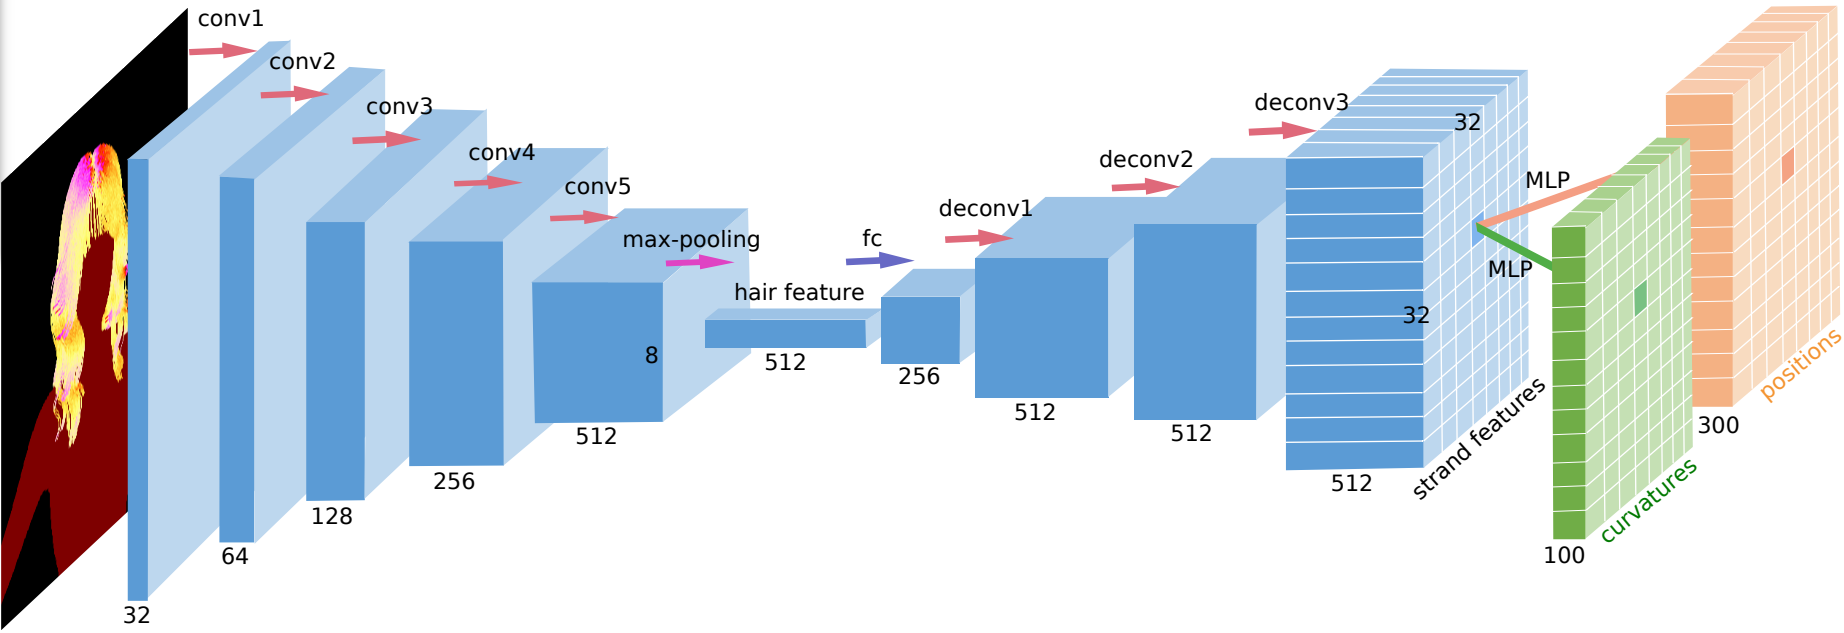
\includegraphics[width=0.8\linewidth]{assets/figures/baselines/HairNet.png}
        \caption{Zhou et al. 2018\cite{Zhou2018SingleViewHR}}
        \label{fig:hairnet}
    \end{figure}
\end{frame}


\subsection{3D Hair Synthesis}
\begin{frame}\frametitle{Related Works}
    \framesubtitle{3D Hair Synthesis}

    \normalsize{\textcolor{myBlue}{\emph{3D Hair Synthesis using Volumetric Variational Autoencoders}}}
    
    \begin{figure}[ht]
        \centering
        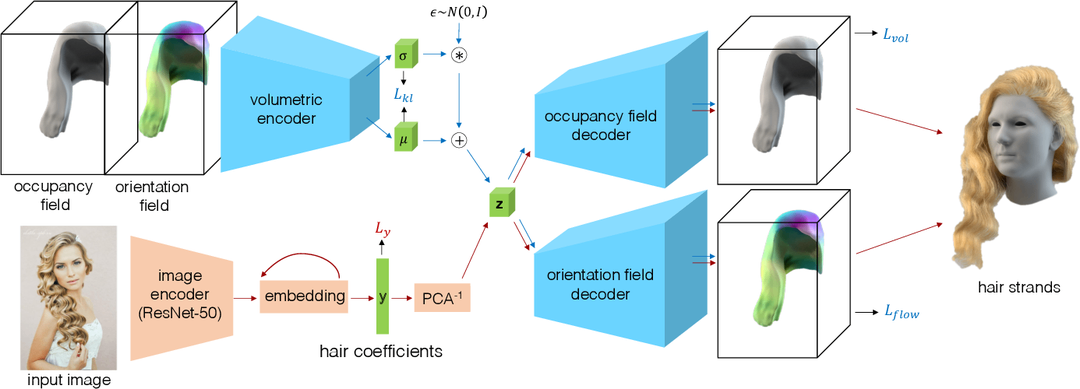
\includegraphics[width=0.8\linewidth]{assets/figures/baselines/3DHairSynthesis.png}
        \caption{Saito et al. 2018\cite{Saito20183DHS}}
        \label{fig:3dhairsynthesis}
    \end{figure}
\end{frame}


\subsection{NeuralHDHair}
\begin{frame}\frametitle{Related Works}
    \framesubtitle{NeuralHDHair}

    \normalsize{\textcolor{myBlue}{\emph{NeuralHDHair: Automatic High-fidelity Hair Modeling from a Single Image Using Implicit Neural Representations}}}
    
    \begin{figure}[ht]
        \centering
        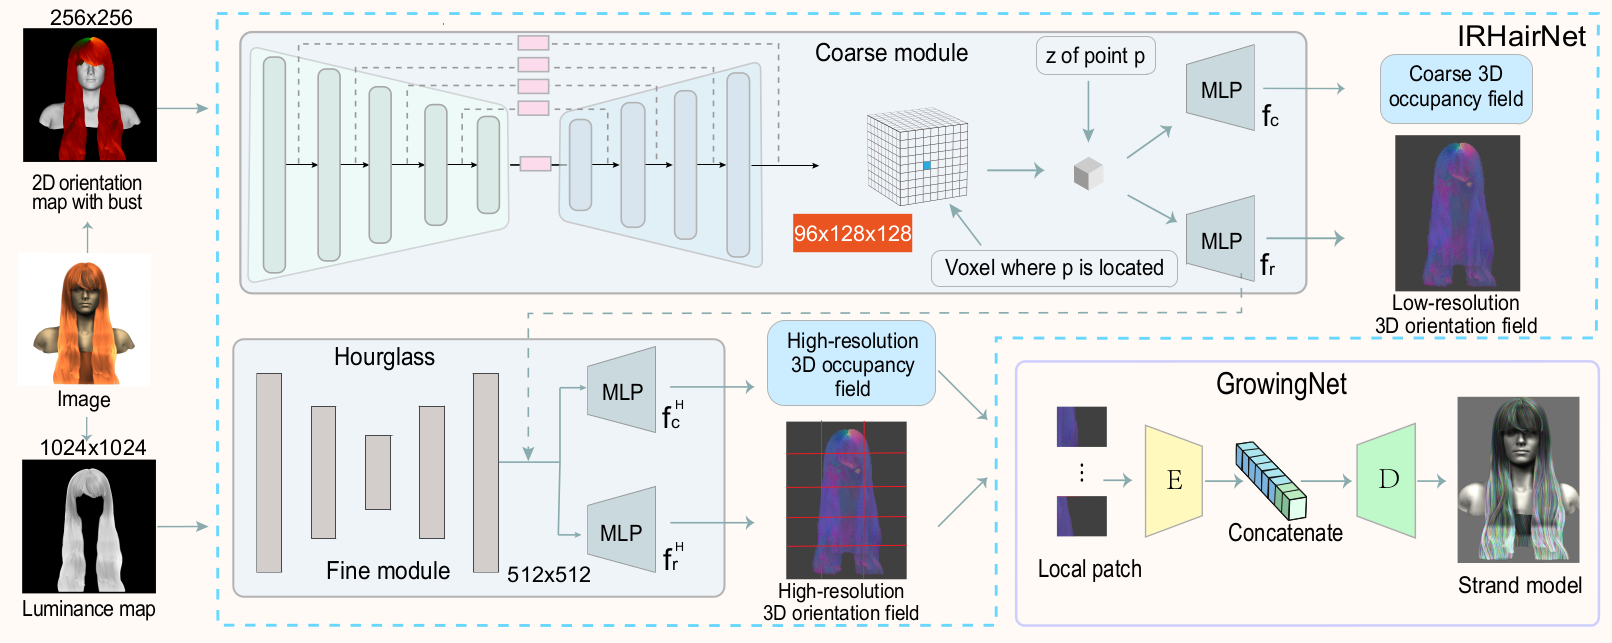
\includegraphics[width=0.8\linewidth]{assets/figures/baselines/NeuralHDHair.png}
        \caption{Wu et al. 2022\cite{wu2022neuralhdhair}}
        \label{fig:neuralhdhair}
    \end{figure}
\end{frame}



\newSection{Motivation}

%---------------------------------------------------------
\begin{frame}[t]{Motivation}
    \textbf{Main Challenge:} Using synthetic data as a prior for real-world 3D hair modeling introduces a domain gap.
\end{frame}

%---------------------------------------------------------
\begin{frame}[t]{Motivation}
    \textbf{Main Challenge:} Using synthetic data as a prior for real-world 3D hair modeling introduces a domain gap.

    \vspace{1em}
    \textbf{Existing Solutions:} 
    \begin{itemize}
        \item Utilize undirected 2D orientation maps as an intermediate representation between the input image and the 3D hair model.
    \end{itemize}
\end{frame}

%---------------------------------------------------------
\begin{frame}[t]{Motivation}
    \textbf{Main Challenge:} Using synthetic data as a prior for real-world 3D hair modeling introduces a domain gap.

    \vspace{1em}
    \textbf{Existing Solutions:} 
    \begin{itemize}
        \item Utilize undirected 2D orientation maps as an intermediate representation between the input image and the 3D hair model.
    \end{itemize}

    \vspace{1em}
    \textbf{Limitations:}
    \begin{itemize}
        \item Ambiguous directionality: Loses 3D cues from the image.
        \item Reliance on image filters: Adds noise and inaccuracies.
    \end{itemize}
\end{frame}

%---------------------------------------------------------
\begin{frame}{Motivation -- Visualization}
    \begin{figure}
        \centering
        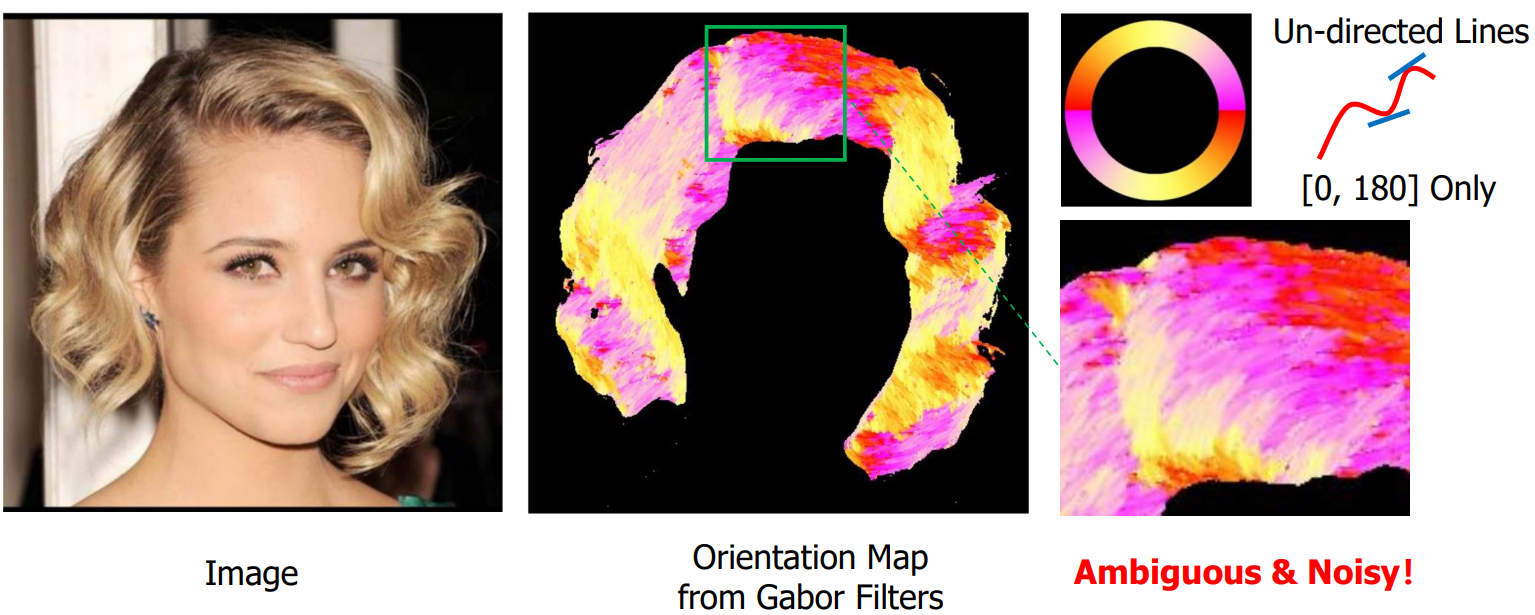
\includegraphics[width=0.9\linewidth]{assets/figures/motivations/orientation-map.png}
        \caption{Example of a 2D orientation map used in existing solutions.}
        \label{fig:motivation-orientation-map}
    \end{figure}
\end{frame}


\newSection{Contribution}

\begin{frame}[t]{Contribution}
    \begin{itemize}
        \item Proposed \emph{HairStep}, a novel intermediate representation combining strand maps and depth maps for 3D hair reconstruction.
        \item Developed a weakly-supervised domain adaptation method for depth estimation using synthetic priors and real-world sparse annotations.
        \item Created \emph{HiSa} (strand annotations) and \emph{HiDa} (relative depth annotations) datasets for 1,250 real portrait images.
        \item Introduced new metrics, \emph{HairSale} (strand alignment error) and \emph{HairRida} (relative depth accuracy), for quantitative evaluation of 3D hair modeling.
        \item Achieved state-of-the-art performance in single-view 3D hair modeling.
    \end{itemize}
\end{frame}

\newSection{HairStep}

%---------------------------------------------------------
\subsection{HairStep Representation}
%---------------------------------------------------------

\begin{frame}[t]{HairStep Representation}
    \textit{HairStep} is defined as $\mathbf{H} = \{\mathbf{O}, \mathbf{D}\}$ for each input image $\mathbf{I} \in \mathbb{R}^{W \times H \times 3}$, where:
    \begin{itemize}
        \item $\mathbf{O} \in \mathbb{R}^{W \times H \times 3}$ is the \emph{Strand Map}.
        \item $\mathbf{D} \in \mathbb{R}^{W \times H \times 1}$ is the \emph{Depth Map}.
    \end{itemize}

    \begin{figure}[t]
        \centering
        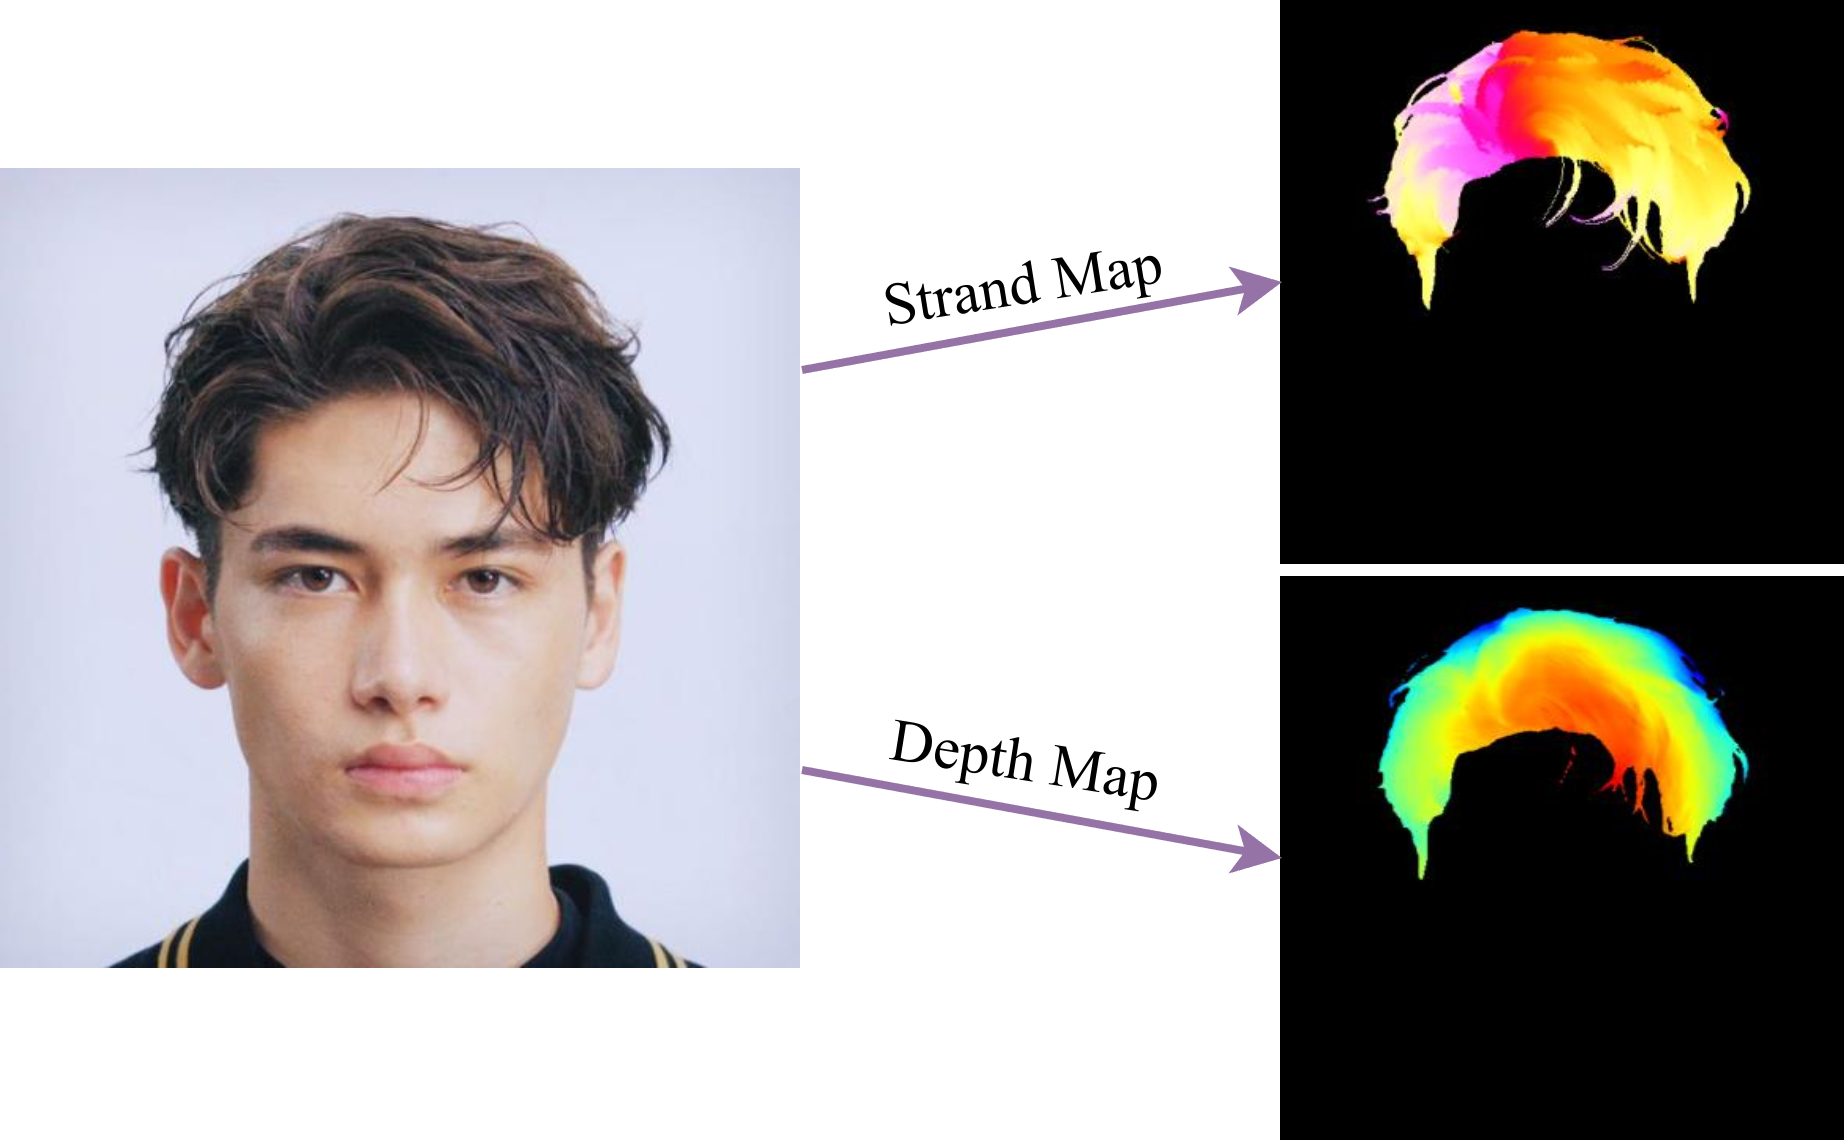
\includegraphics[width=0.45\textwidth]{assets/figures/method/hairstep.png}
        \caption{Example of the HairStep representation.}
        \label{fig:hairstep_rep}
    \end{figure}
\end{frame}

%---------------------------------------------------------
\begin{frame}[t]{HairStep Representation -- Strand Map}
    \textit{Strand Map} $\mathbf{O} \in \mathbb{R}^{W \times H \times 3}$ is defined at each pixel $x$ as
    \begin{equation}
        \mathbf{O}(x) = \bigl(\mathbf{M}(x),\; \tfrac{\mathbf{O}_{\mathrm{2D}}(x)}{2} + 0.5\bigr),
        \label{eq:strand_map}
    \end{equation}
    where:
    \begin{itemize}
        \item $\mathbf{M}(x) \in \{0, 1\}$ is a hair mask (1 denotes hair, 0 denotes background).
        \item $\mathbf{O}_{\mathrm{2D}}(x) \in \mathbb{R}^2$ is the unit vector of 2D hair-growth orientation.
    \end{itemize}
    
    \begin{figure}[t]
        \centering
        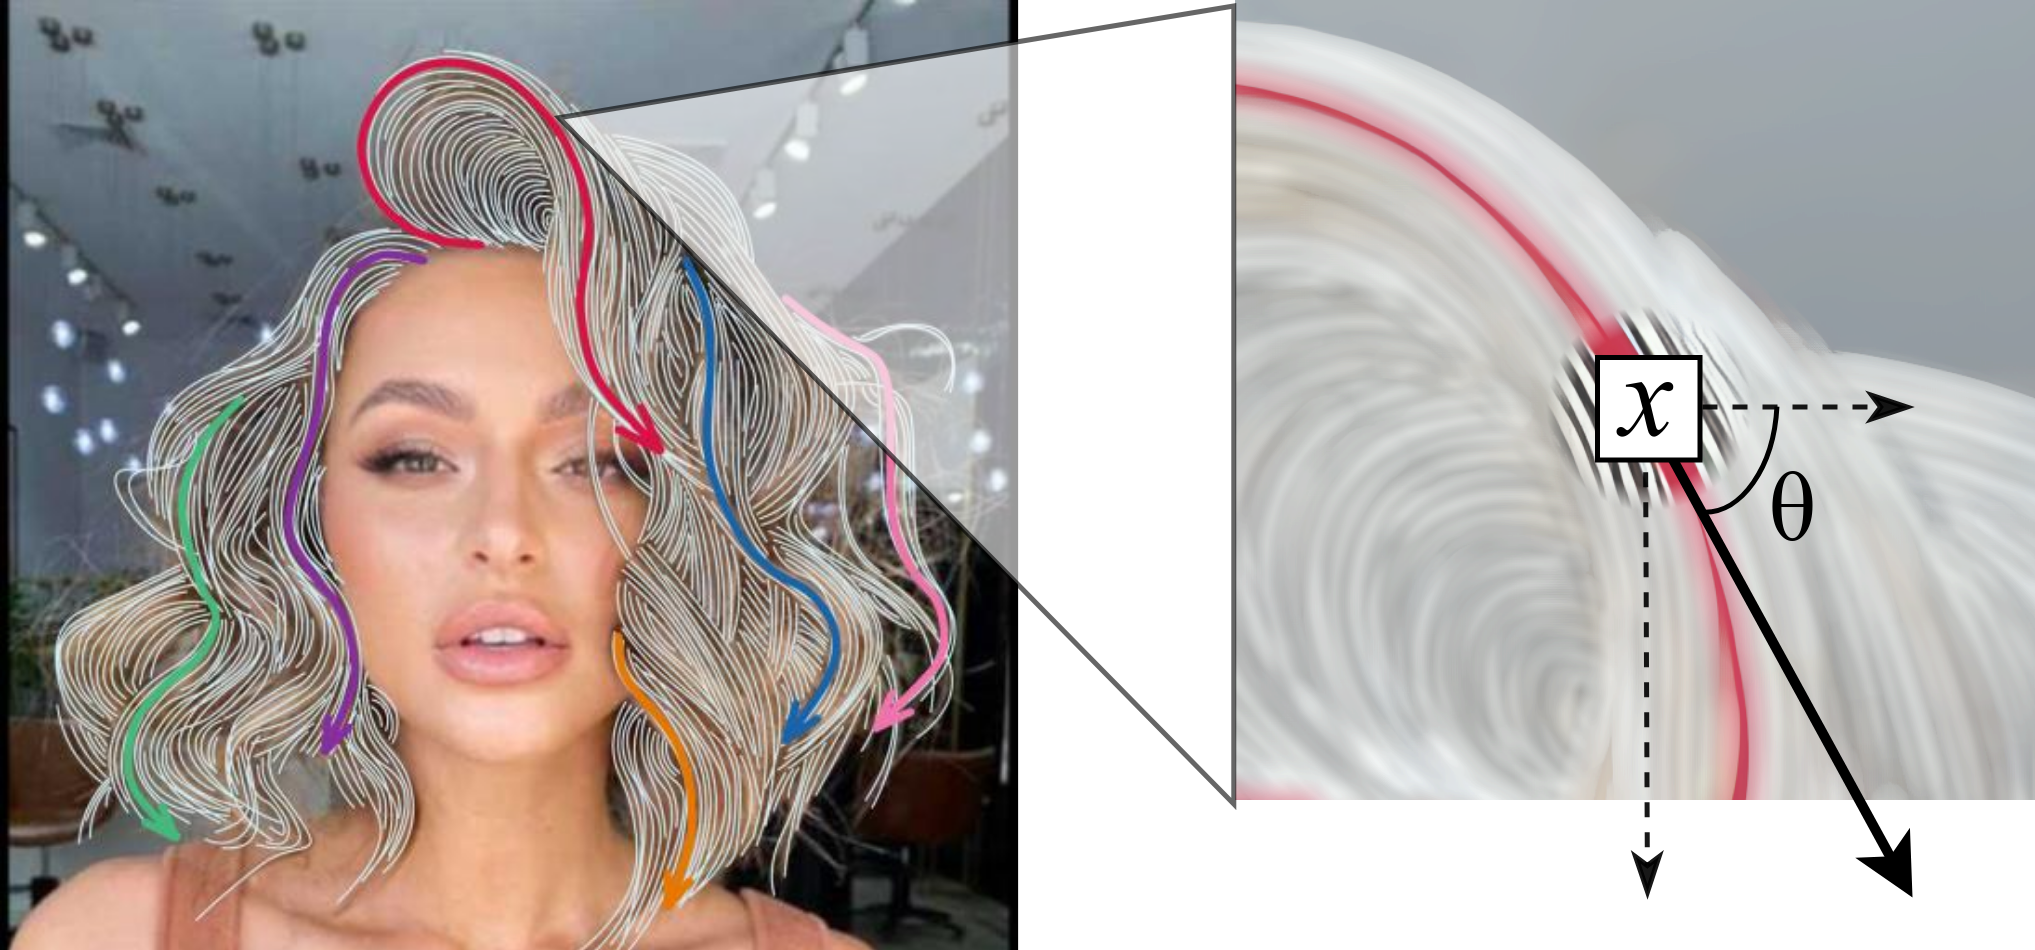
\includegraphics[width=0.45\textwidth]{assets/figures/method/hisa/o_2d.png}
        \caption{Visualization of $\mathbf{O}_{\mathrm{2D}}(x)$, where 
        $\mathbf{O}_{\mathrm{2D}}(x) = \begin{bmatrix}\cos(\theta) \\ -\sin(\theta)\end{bmatrix}$.}
        \label{fig:o_2d_example}
    \end{figure}
\end{frame}

%---------------------------------------------------------
\begin{frame}[t]{HairStep Representation -- Depth Map}
    The \emph{Depth Map} $\mathbf{D} \in \mathbb{R}^{W \times H \times 1}$ defines
    relative depth differences among hair strands.

    \begin{itemize}
        \item Each pixel $\mathbf{D}(x) \in [0, 1]$:
        \begin{itemize}
            \item $\mathbf{D}(x) = 0$: Farthest from the camera (or background, where $\mathbf{M}(x)=0$).
            \item $\mathbf{D}(x) = 1$: Closest to the camera.
        \end{itemize}
    \end{itemize}  % <-- end the outer itemize before starting the figure environment

    \begin{figure}[t]
        \centering
        
\includegraphics[width=0.55\textwidth]{assets/figures/method/depth-map/depth-map.png}
        \caption{Example of the depth map $\mathbf{D}(x)$.}
        \label{fig:depth_map_example}
    \end{figure}
\end{frame}

%---------------------------------------------------------
\subsection{Overview}
%---------------------------------------------------------

\begin{frame}{Overview}
    \begin{figure}[t]
        \centering
        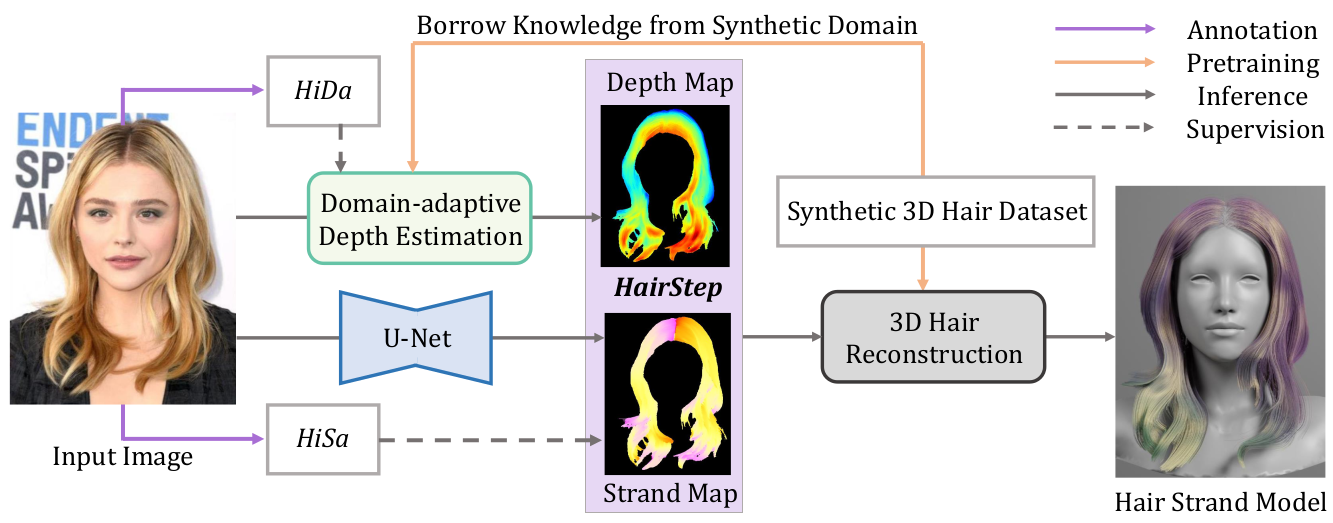
\includegraphics[width=0.95\textwidth]{assets/figures/method/overview.png}
        \caption{The pipeline of single-view 3D hair reconstruction using \textit{HairStep}.}
        \label{fig:overview}
    \end{figure}
\end{frame}

%---------------------------------------------------------
\begin{frame}[t]{Overview}
    The pipeline has three main components:
    \begin{itemize}
        \item \textbf{Strand Map Extraction \& Prediction:} 
        \begin{itemize}
            \item Extract strand maps from real images using the \textit{HiSa} dataset.
        \end{itemize}
        \item \textbf{Domain-Adaptive Depth Estimation:}
        \begin{itemize}
            \item Estimate relative depth from real images using the \textit{HiDa} dataset.
            \item Weakly supervise depth estimation using synthetic data.
        \end{itemize}
        \item \textbf{3D Hair Reconstruction:}
        \begin{itemize}
            \item Reconstruct 3D hair strands from the predicted strand and depth maps.
        \end{itemize}
    \end{itemize}
\end{frame}

%---------------------------------------------------------
\subsection{Strand Map Extraction \& Prediction}
%---------------------------------------------------------

\begin{frame}[t]{Strand Map Extraction}
    Extracting strand maps is crucial for learning-based 3D hair modeling.
    \begin{itemize}
        \item \textbf{Synthetic}: Use rendering techniques (e.g.\cite{liu2019softras}).
        \item \textbf{Real}: Use a U-Net trained on the \textit{HiSa} dataset.
    \end{itemize}
\end{frame}

%---------------------------------------------------------
\begin{frame}[t]{HiSa Dataset}
    The \emph{HiSa} dataset provides strand maps for real images.

    \begin{itemize}
        \item \textbf{Collection:} 1,250 portrait images.
        \item \textbf{Annotation Process:}
        \begin{itemize}
            \item Artists draw directional vector curves from the hair roots to the hair ends.
            \item Vector strokes are colored by the definition of Eq.~\ref{eq:strand_map}.
            \item Colored strokes are interpolated to form the strand map.
        \end{itemize}
        \item \textbf{Statistics:}
        \begin{itemize}
            \item On average, 300 strokes per portrait is annotated.
        \end{itemize}
    \end{itemize}
\end{frame}

%---------------------------------------------------------
\begin{frame}{HiSa Dataset (Visualization)}
    \begin{figure}[t]
        \centering
        \includegraphics[width=0.95\textwidth]{assets/figures/method/hisa/hisa.png}
        \caption{Strand maps extraction steps:
        (a) Portrait image, (b) Annotated vector strokes, (c) Colored strokes, (d) Strand map.}
        \label{fig:hisa}
    \end{figure}
\end{frame}

%---------------------------------------------------------
\begin{frame}{Strand Map Prediction}
    \begin{figure}[t]
        \centering
        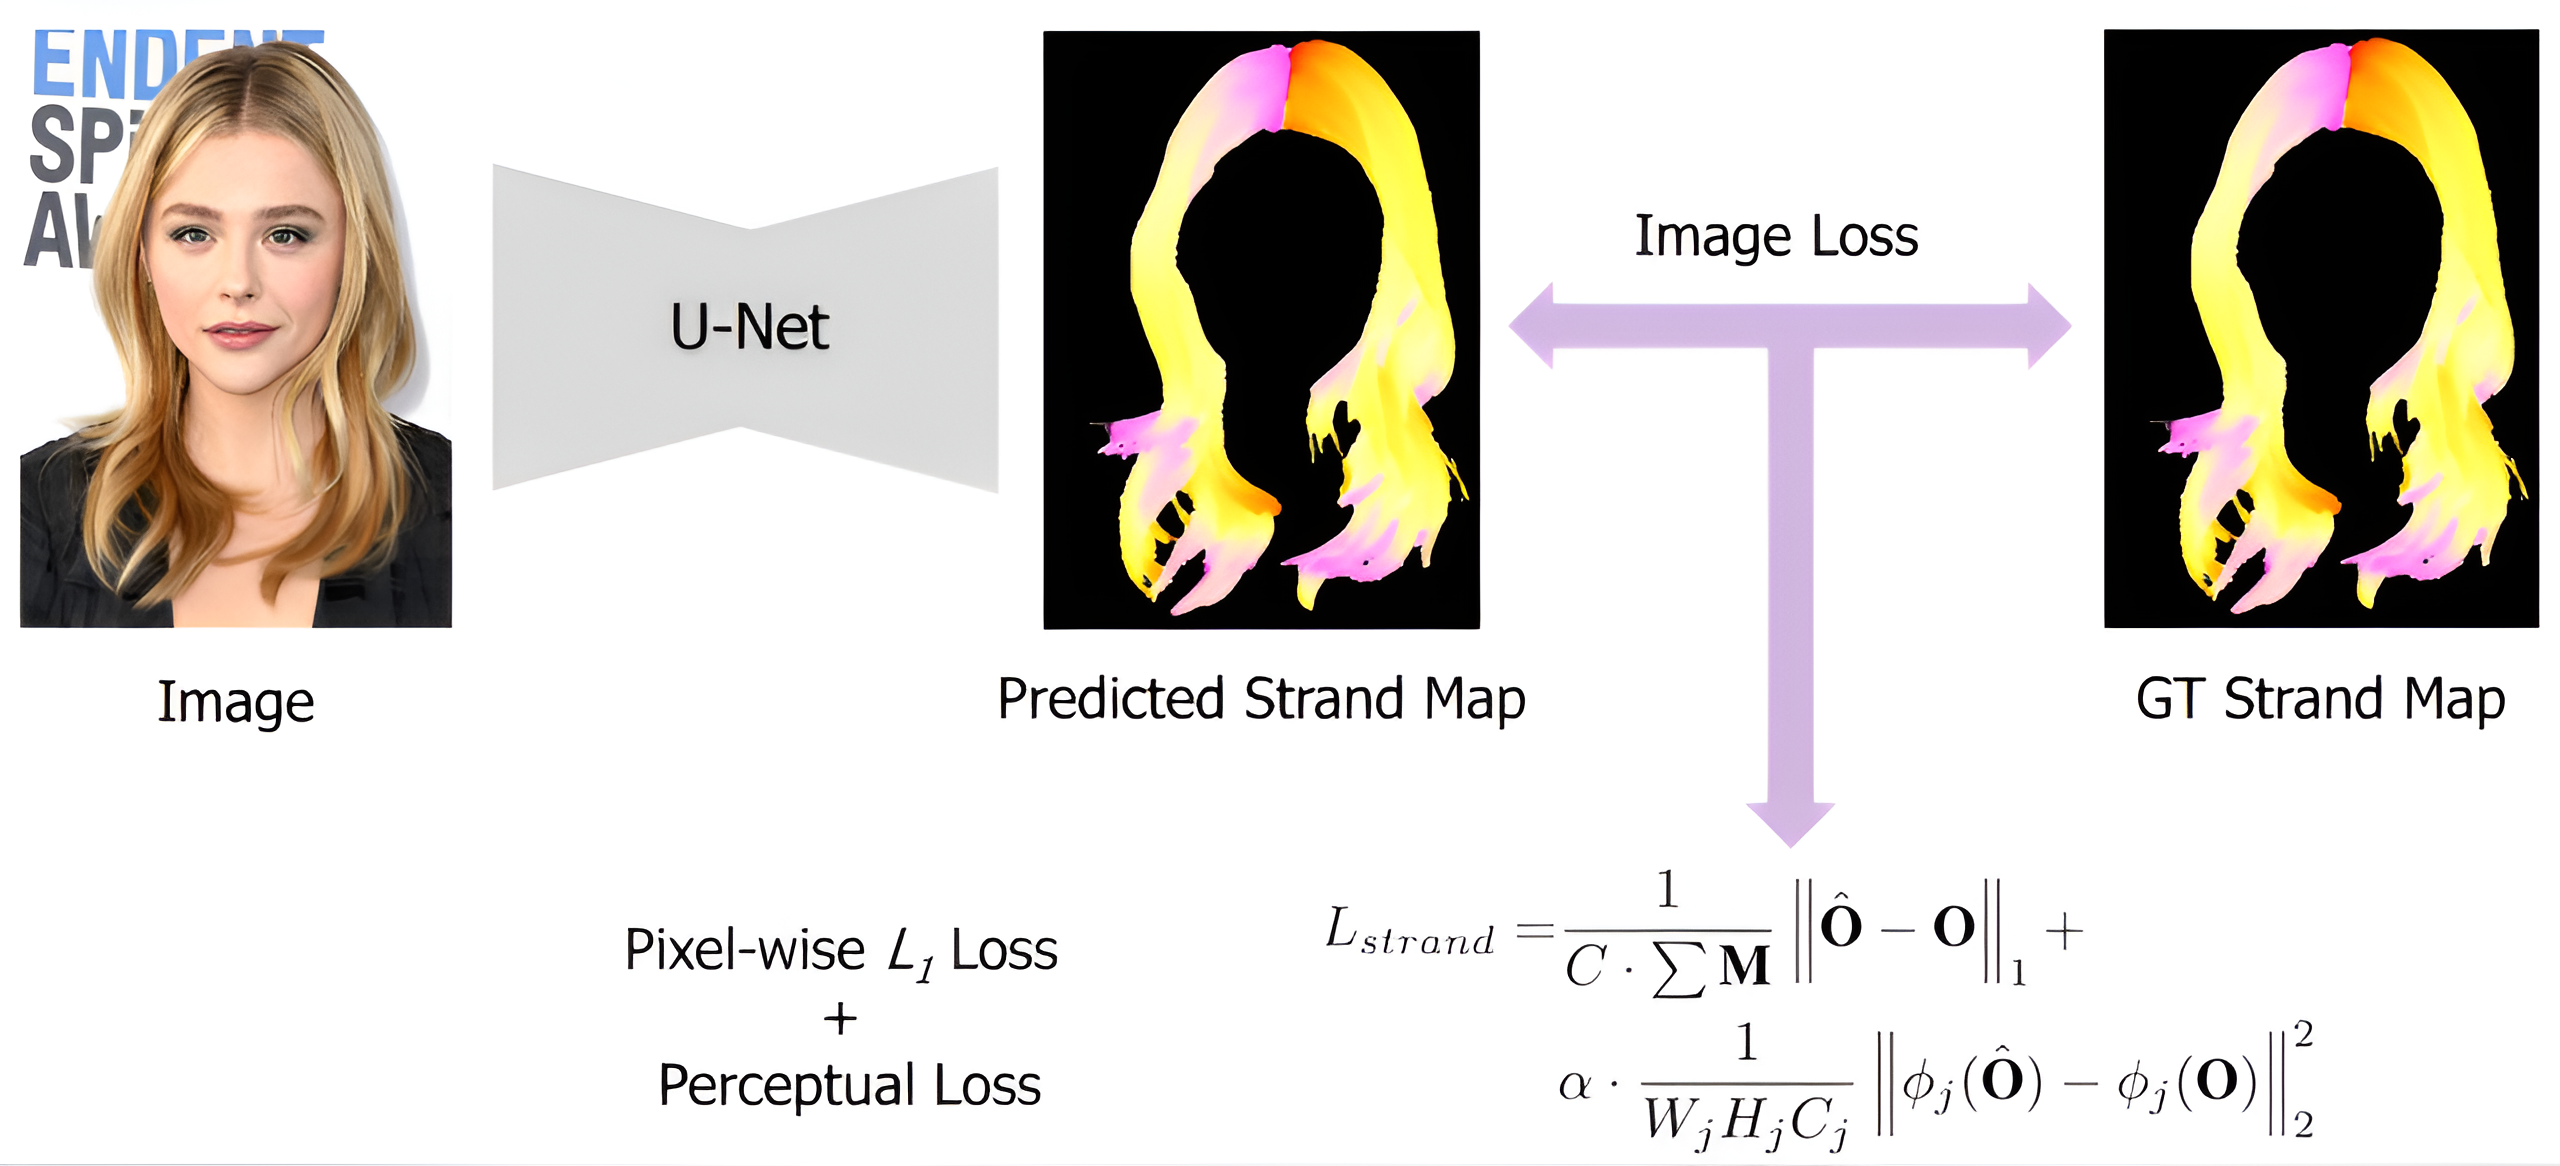
\includegraphics[width=0.95\textwidth]{assets/figures/method/strand/prediction.png}
        \caption{Example pipeline for strand map prediction.}
        \label{fig:strand-map-prediction}
    \end{figure}
\end{frame}

%---------------------------------------------------------
\subsection{Depth Estimation and HiDa Dataset}
%---------------------------------------------------------

\begin{frame}{Relative Depth Estimation}
    Inspired by the depth-in-the-wild approach~\cite{Zhou2018SingleViewHR}, relative depth estimation serves as a weak supervision signal.
    \begin{figure}[t]
        \centering
        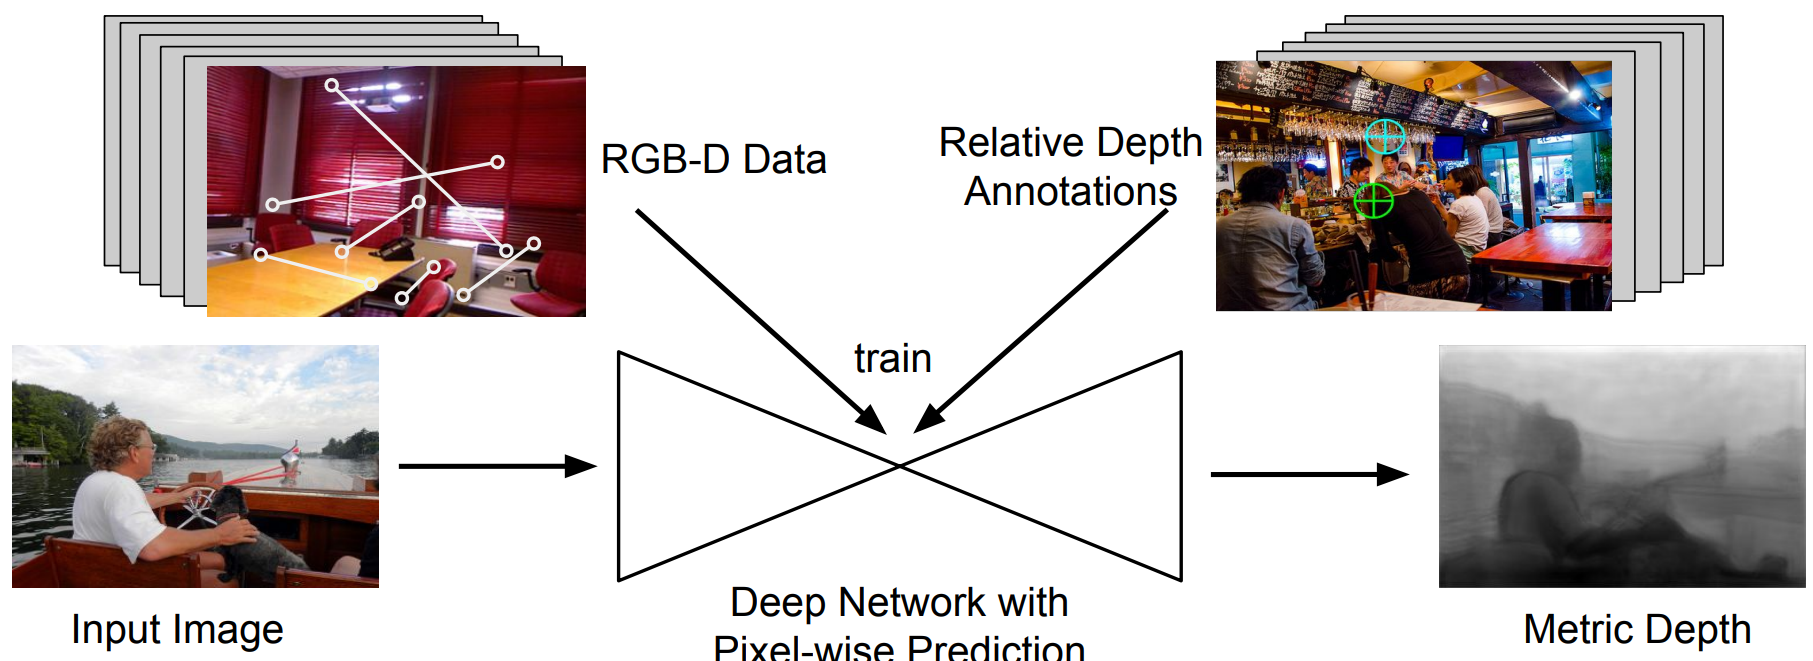
\includegraphics[width=0.85\textwidth]{assets/figures/method/depth/depth-in-the-wild.png}
        \caption{Overview of the depth-in-the-wild pipeline.}
        \label{fig:depth_in_the_wild}
    \end{figure}
\end{frame}

%---------------------------------------------------------
\begin{frame}[t]{HiDa Dataset}
    The \emph{HiDa} dataset provides relative depth annotations for hair regions in real images.

    \begin{itemize}
        \item \textbf{Collection:} 1,250 portrait images (the same as \textit{HiSa}).
        \item \textbf{Annotation Process:}
        \begin{itemize}
            \item Generate super-pixels within the hair region.
            \item Sample pixel pairs from adjacent super-pixels.
            \item Show each pair on the portrait and ask annotators which point is closer.
        \end{itemize}
        \item \textbf{Statistics:}
        \begin{itemize}
            \item On average, 140 pairs per portrait.
            \item 129,079 annotated pixel pairs in total.
        \end{itemize}
    \end{itemize}
\end{frame}


%---------------------------------------------------------
\begin{frame}[t]{HiDa Dataset (Visualization)}
    \begin{figure}[t]
        \centering
        \includegraphics[width=0.8\textwidth]{assets/figures/method/hida/superpixel.png}
        \caption{Example of super-pixels generated for the HiDa dataset.}
        \label{fig:hida-superpixel}
    \end{figure}
\end{frame}

%---------------------------------------------------------
\begin{frame}{Domain-Adaptive Depth Estimation}
    \begin{figure}[t]
        \centering
        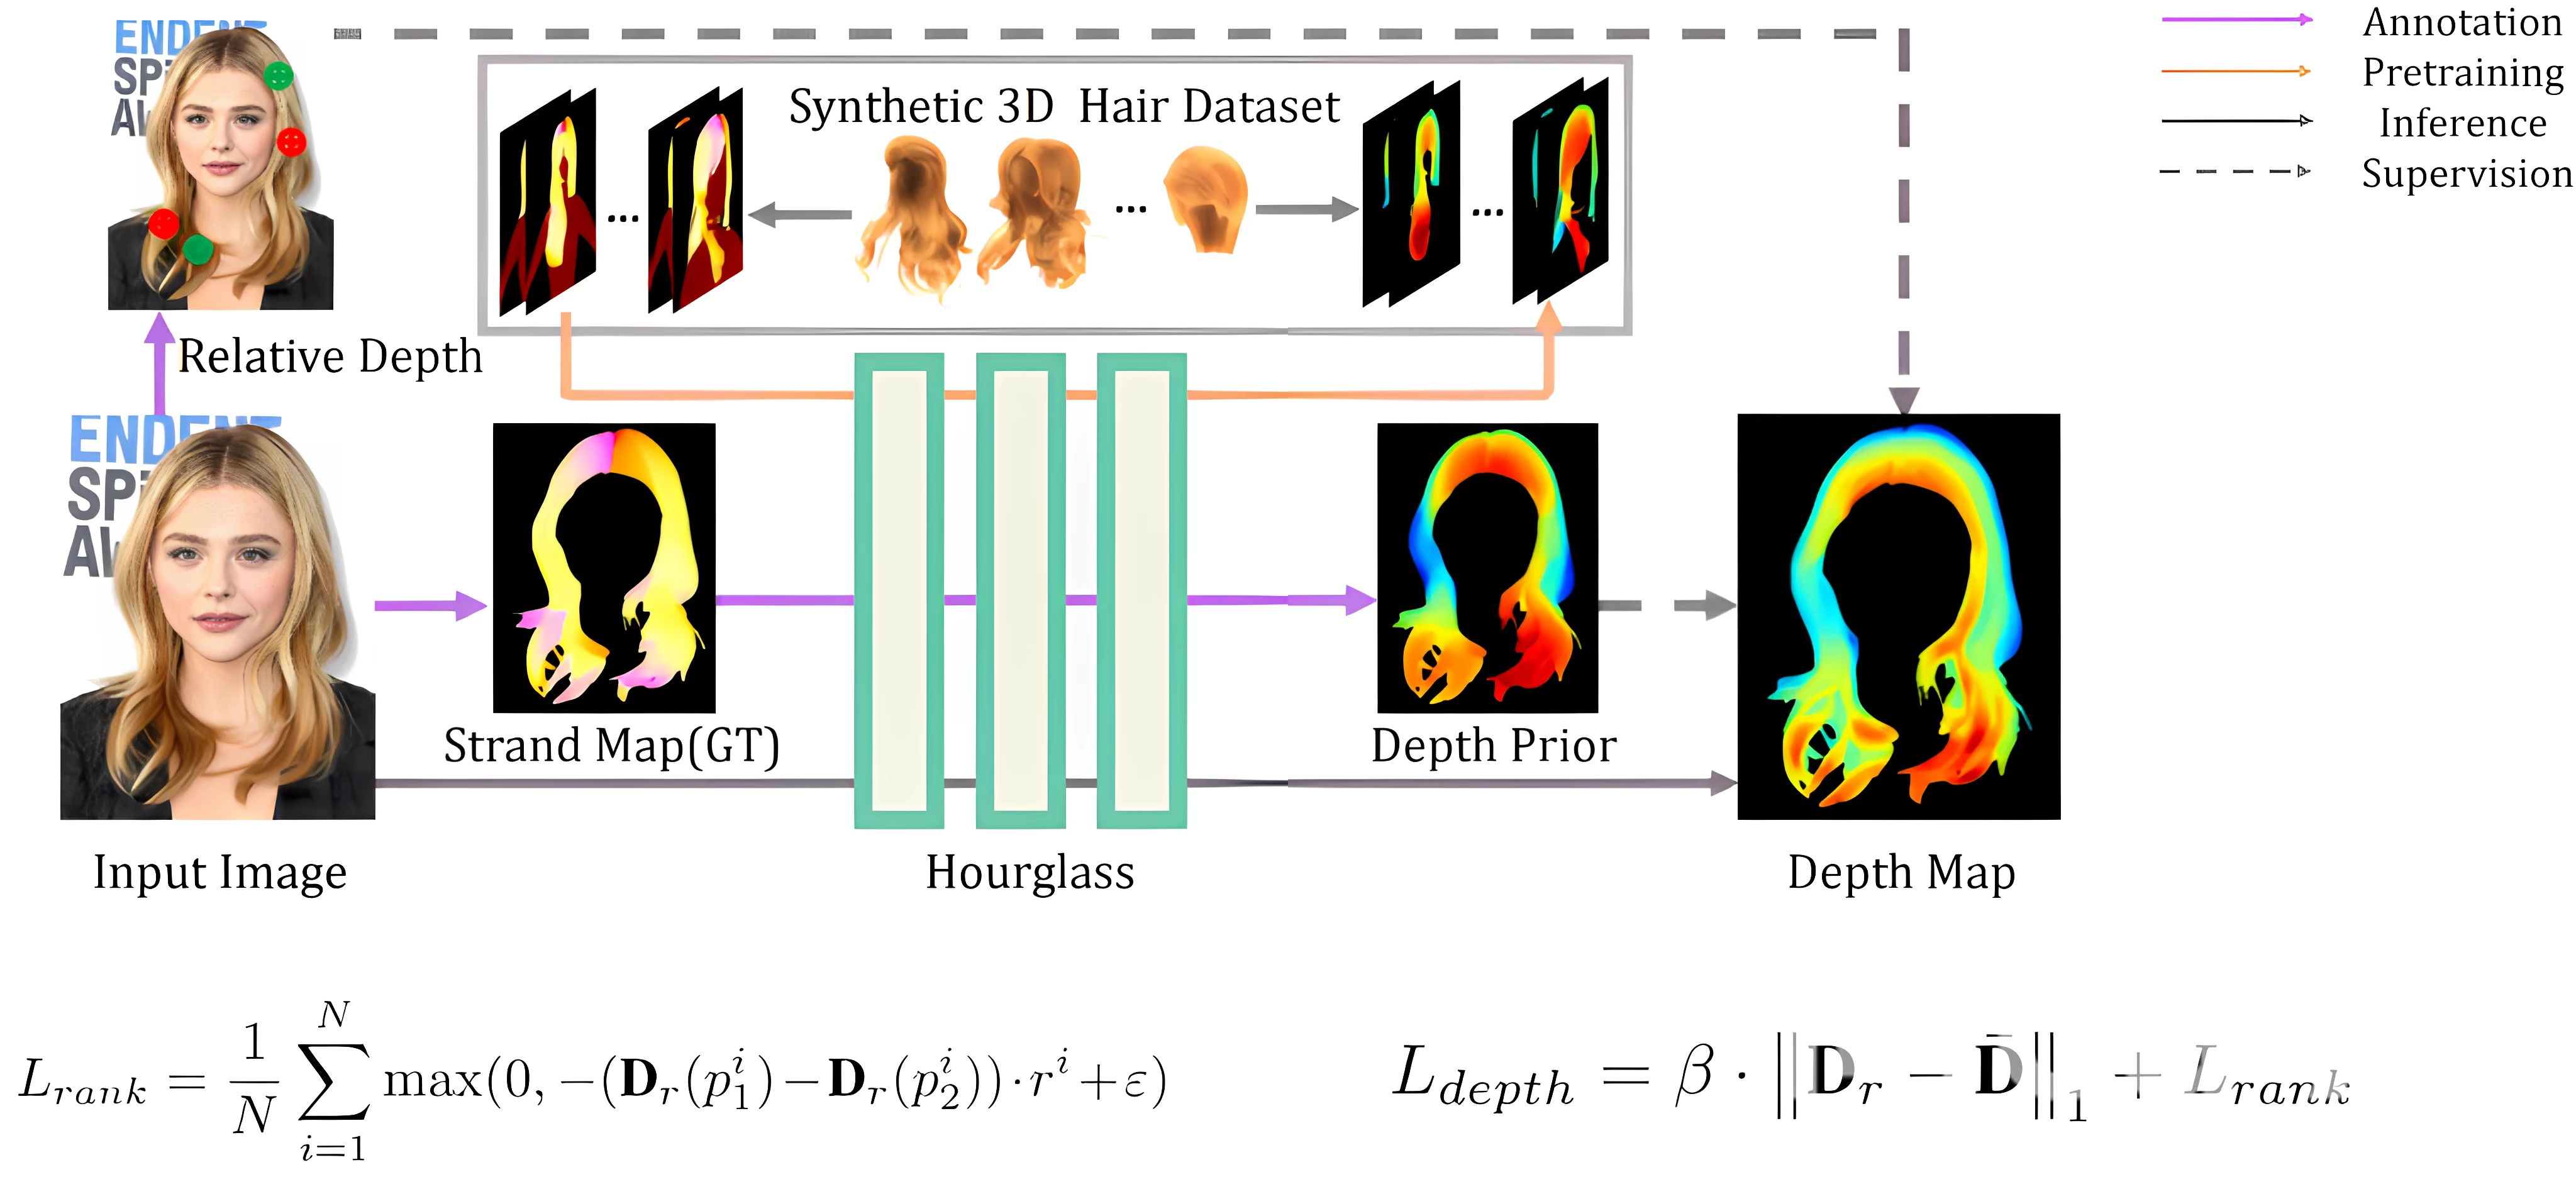
\includegraphics[width=0.9\textwidth]{assets/figures/method/depth/pipeline.png}
        \caption{Overview of the domain-adaptive depth estimation approach.}
        \label{fig:depth_estimation_overview}
    \end{figure}
\end{frame}

%---------------------------------------------------------
\begin{frame}{Depth Estimation}
    We use an \emph{Hourglass} network to predict depth maps from input images. 
    A margin-based ranking loss is applied for relative depth estimation.
    \begin{figure}[t]
        \centering
        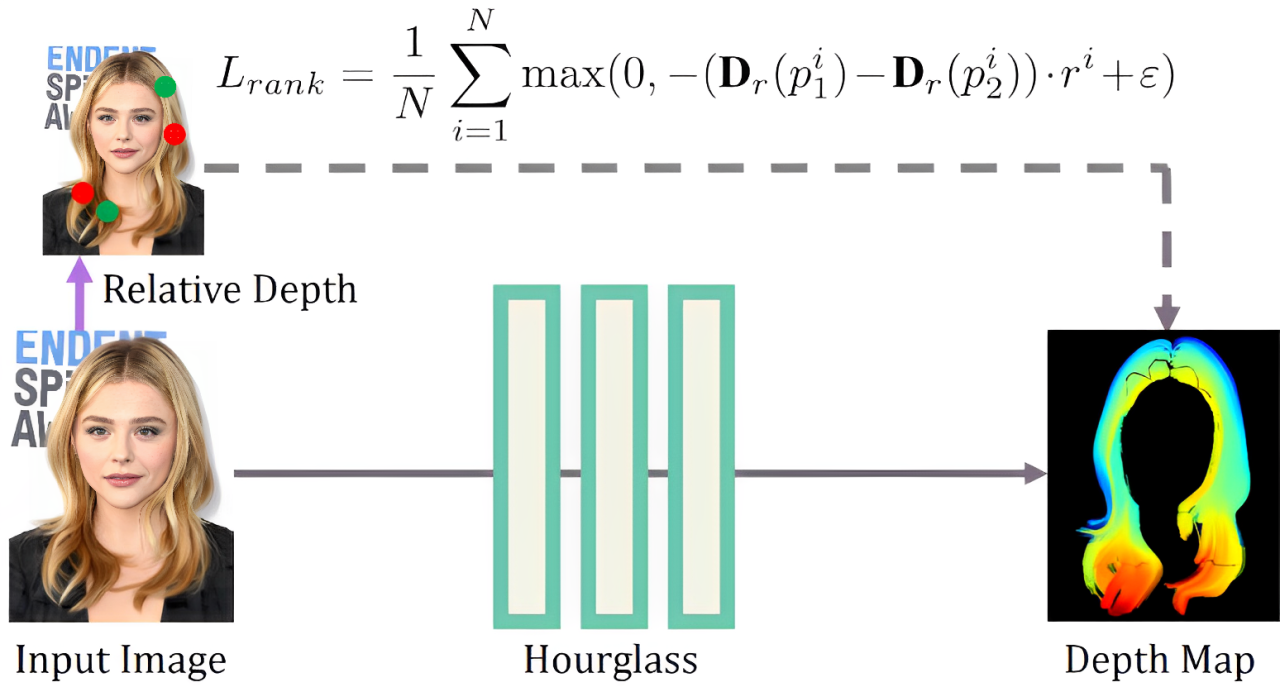
\includegraphics[width=0.6\textwidth]{assets/figures/method/depth/hourglass.png}
        \caption{Each pair $(p^i_1, p^i_2)$ forms the $i$-th annotated pair; $r^i=1$ if $p^i_1$ is closer, $r^i=-1$ otherwise.}
        \label{fig:hourglass_depth}
    \end{figure}
\end{frame}

%---------------------------------------------------------
\begin{frame}[t]{Depth Estimation Challenges}
    Training with only ordinal labels can introduce ambiguity and artifacts in depth prediction, resulting in noisy or coarse 3D hair models.
    \vspace{0.5em}
    \begin{figure}[t]
        \centering
        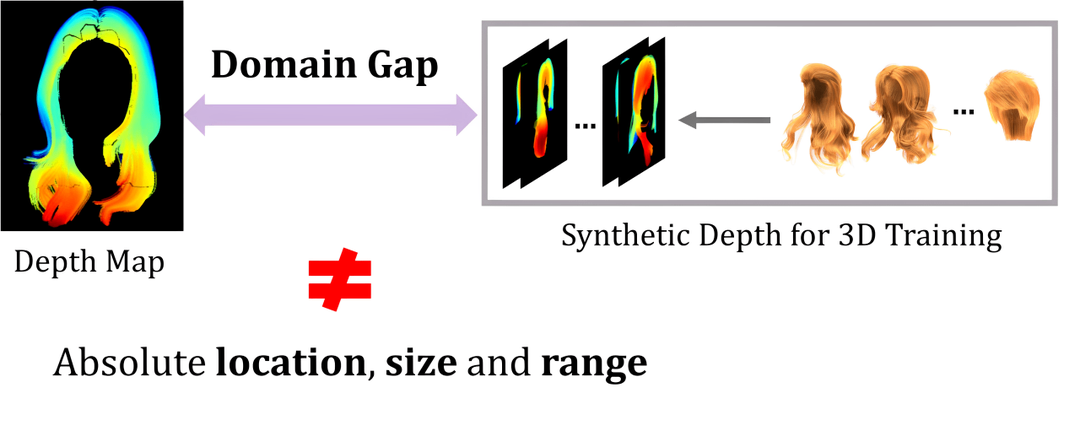
\includegraphics[width=0.6\textwidth]{assets/figures/method/depth/domain-gap.png}
        \caption{Domain gaps and artifacts in predicted depth from ordinal labels.}
        \label{fig:domain_gap}
    \end{figure}
\end{frame}

%---------------------------------------------------------
\begin{frame}[t]{Domain-Adaptive Depth Estimation}
    To mitigate artifacts, a domain-adaptive depth estimation pipeline refines depth predictions using synthetic data:
    \begin{itemize}
        \item \textbf{Pre-training} a Hourglass network \texttt{Depth\_syn} on synthetic data:
        \begin{itemize}
            \item Input: Ground-truth strand map.
            \item Output: Depth map $\bar{\mathbf{D}}$.
            \item Loss: $L_1$ loss on $\bar{\mathbf{D}}$.
        \end{itemize}
        \item \textbf{Training} a Hourglass network \texttt{Depth\_r} on real data:
        \begin{itemize}
            \item Input: Real images + ground-truth strand map.
            \item Output: Depth map $\mathbf{D}_r$.
            \item Supervision: Depth prior $\bar{\mathbf{D}}$ from \texttt{Depth\_syn}.
            \item Final Loss: $L_{\text{depth}} = \beta \|\mathbf{D}_r - \bar{\mathbf{D}}\|_1 + L_{\text{rank}}$.
        \end{itemize}
    \end{itemize}
\end{frame}

%---------------------------------------------------------
\subsection{Single-View 3D Hair Modeling}
%---------------------------------------------------------

\begin{frame}[t]{Single-View 3D Hair Modeling}
    \begin{figure}[t]
        \centering
        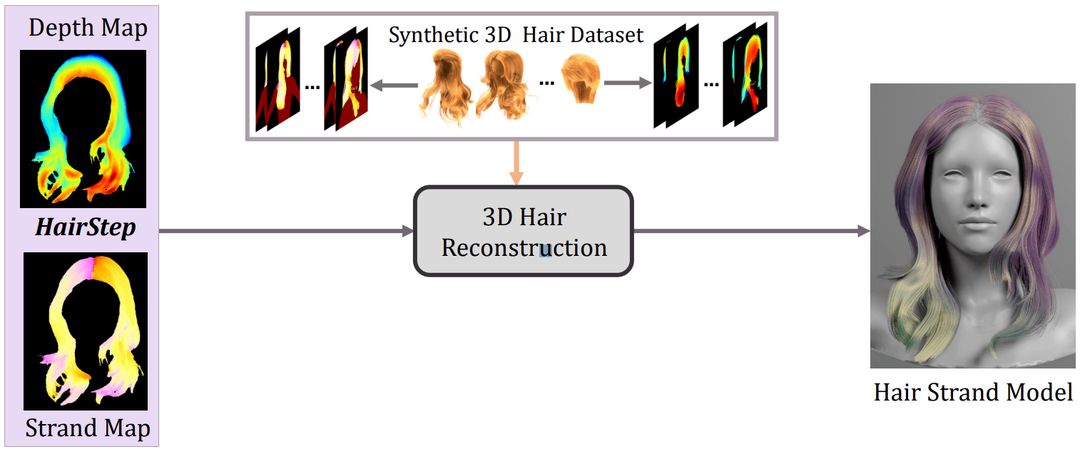
\includegraphics[width=0.9\textwidth]{assets/figures/method/reconstruction.png}
        \caption{Pipeline for single-view 3D hair modeling using \emph{HairStep}.}
        \label{fig:single_view_3d_hair_modeling}
    \end{figure}
\end{frame}

%---------------------------------------------------------
\begin{frame}[t]{Single-View 3D Hair Modeling Details}
    \textbf{Objective:} Reconstruct strand-level 3D hair from a \emph{single-view} portrait image via the \emph{HairStep} representation $\{\mathbf{O}, \mathbf{D}\}$.
    \begin{itemize}
        \item \textbf{Key Idea:} Convert HairStep into \emph{implicit fields} encoding 3D hair geometry.
        \item \textbf{Two Main Stages}:
        \begin{itemize}
            \item \textbf{Implicit Representation:} Predict occupancy and orientation fields in a canonical head space.
            \item \textbf{Strand Generation:} Convert those fields into explicit 3D hair strands.
        \end{itemize}
    \end{itemize}
\end{frame}

%---------------------------------------------------------
\begin{frame}[t]{Implicit 3D Hair Representation}
    \textbf{Why Implicit Fields?}
    \begin{itemize}
        \item Flexible, memory-efficient for complex volumetric structures like hair.
        \item Smoothly captures continuous geometry and orientations without enumerating every strand.
    \end{itemize}

    \textbf{Following NeuralHDHair~\cite{wu2022neuralhdhair}, define:}
    \begin{itemize}
        \item \textbf{Occupancy Field} $f_{\text{occ}}(v) \in [0,1]$:
        \begin{itemize}
            \item Indicates inside vs.\ outside the hair volume.
            \item $f_{\text{occ}}(v) = 1$ if $v$ is inside hair; $0$ otherwise.
        \end{itemize}
        \item \textbf{Orientation Field} $f_{\text{orient}}(v) \in \mathbb{R}^3$:
        \begin{itemize}
            \item Unit vector of local hair-growth direction inside hair volume.
            \item Zero vector outside.
        \end{itemize}
    \end{itemize}
\end{frame}

%---------------------------------------------------------
\begin{frame}[t]{Neural Network Prediction (NeuralHDHair)}
    \textbf{NeuralHDHair*} \emph{(adapted from~\cite{wu2022neuralhdhair})}
    \begin{itemize}
        \item \textbf{Input:} Strand map $\mathbf{O}$ and depth map $\mathbf{D}$ (4-channel input including hair mask).
        \item \textbf{Output:} Implicit occupancy $f_{\text{occ}}(\mathbf{x})$ and orientation $f_{\text{orient}}(\mathbf{x})$ fields.
        \item \textbf{Modifications:}
        \begin{itemize}
            \item \emph{No Luminance Map}: Reduces domain gap from lighting differences.
            \item \emph{Omit GrowingNet}: Focus on reconstruction quality using direct strand-growing from implicit fields.
        \end{itemize}
    \end{itemize}
\end{frame}

%---------------------------------------------------------
\begin{frame}[t]{Hair Strand Generation}
    After predicting the implicit fields, hair strands are generated following DeepSketchHair~\cite{shen2020deepsketchhair}:
    \begin{itemize}
        \item \textbf{Initialization:}
        \begin{itemize}
            \item Place hair roots on a standard scalp model.
        \end{itemize}
        \item \textbf{Strand Growing:}
        \begin{itemize}
            \item From each root, follow $f_{\text{orient}}$.
            \item Stop when $f_{\text{occ}} = 0$ or reaching max length.
        \end{itemize}
        \item \textbf{Result:}
        \begin{itemize}
            \item A dense set of 3D hair strands ($\sim$10K strands) replicating the input hairstyle.
        \end{itemize}
    \end{itemize}
\end{frame}


\newSection{Experiments}

% Slide 1: Outline
\begin{frame}[t]{Experiments: Outline}
    \begin{itemize}
        \item \textbf{Evaluation Metrics:} Synthetic vs. real benchmarks, new metrics (\emph{HairSale}, \emph{HairRida}).
        \item \textbf{Datasets:} Synthetic (USC-HairSalon) and real (\emph{HiSa}, \emph{HiDa}).
        \item \textbf{Implementation Details:} Network architecture, training setup, sampling strategy.
        \item \textbf{Quantitative Results:} Comparisons with state-of-the-art methods on synthetic \& real images.
        \item \textbf{Ablation Studies:} Role of strand map, depth map, and other design choices.
        \item \textbf{Limitations \& Future Work:} Rare hairstyles, annotation constraints.
    \end{itemize}
\end{frame}

\begin{frame}[t]{Evaluation Metrics}
    \begin{itemize}
        \item \textbf{Quantitative:}
        \begin{itemize}
            \item \textbf{\emph{HairSale} (Strand Metric):}
            \begin{itemize}
                \item Mean angle error of growing directions.
            \end{itemize}
            \item \textbf{\emph{HairRida} (Depth Metric):}
            \begin{itemize}
                \item Relative depth accuracy for pixel pairs in \emph{HiDa}.
            \end{itemize}
        \end{itemize}
        \item \textbf{Qualitative:}
        \begin{itemize}
            \item Only Comparisons of the Visual Quality in Existing Methods.
            \item User Study (Limited).
        \end{itemize}
    \end{itemize}
\end{frame}


\begin{frame}{Evaluation Metrics -- Qualitative}
    \begin{figure}
        \centering
        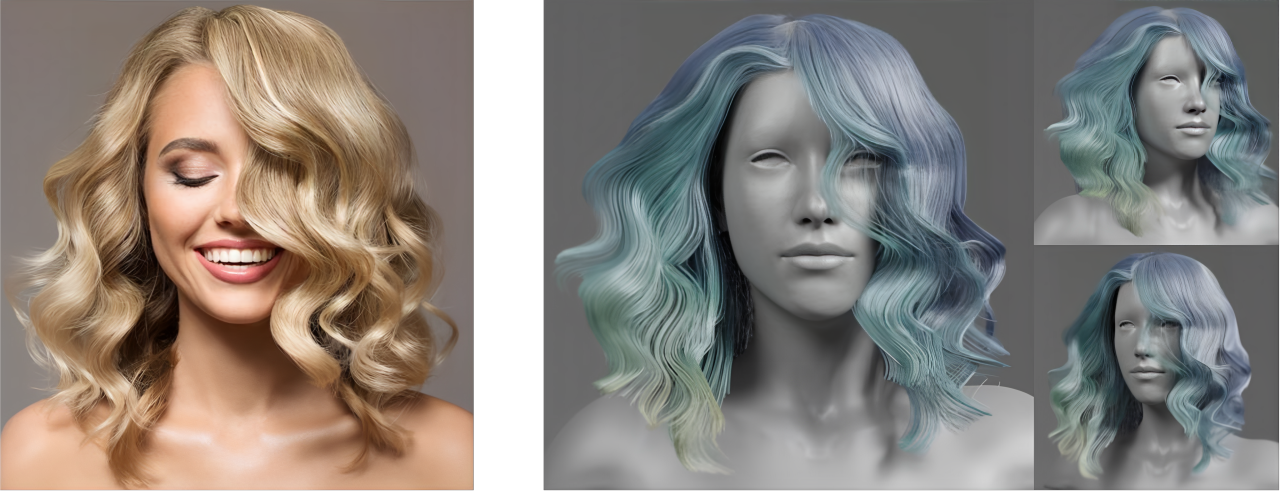
\includegraphics[width=0.9\textwidth]{assets/figures/eval/metrics/input-output.png}
    \end{figure}
\end{frame}

\begin{frame}[t]{Evaluation Metrics -- HairSale}
    \textbf{HairSale: Mean Angle Error of Growing Direction}
    \begin{equation*}
        \text{HairSale} = \frac{1}{K} \sum_{i} \arccos\left( V(O_r(x_i)) \cdot V(O_{gt}(x_i)) \right)
    \end{equation*}
    \begin{itemize}
        \item \textbf{Components:}
        \begin{itemize}
            \item \(U\): Intersected region of rendered mask and ground-truth.
            \item \(K\): Total pixels in \(U\).
            \item \(V(O_r(x_i))\): Unit vector at pixel \(x_i\) in rendered strand map.
            \item \(V(O_{gt}(x_i))\): Unit vector at pixel \(x_i\) in ground-truth strand map.
        \end{itemize}
        \item \textbf{Range:} 0 to 180 degrees.
    \end{itemize}
\end{frame}


\begin{frame}[t]{Evaluation Metrics -- HairRida}
    \textbf{HairRida: Relative Depth Accuracy}
    \begin{equation*}
        \text{HairRida} = \frac{1}{Q} \sum_{i} \max(0, r_i \cdot \text{sign}(D_r(p_{i1}) - D_r(p_{i2})))
    \end{equation*}
    \begin{itemize}
        \item \textbf{Components:}
        \begin{itemize}
            \item \(U\): Intersected region of rendered mask and ground-truth.
            \item \(Q\): Total number of pixel pairs in \(U\).
            \item \(r_i\): Ground-truth relative depth order.
            \item \(D_r(p_{i1})\), \(D_r(p_{i2})\): Depth values at pixel pair \(p_{i1}\) and \(p_{i2}\) in rendered depth map.
        \end{itemize}
    \end{itemize}
\end{frame}

\begin{frame}[t]{Evaluation Metrics -- Quantitative}
    \begin{figure}
        \centering
        \includegraphics[width=0.95\textwidth]{assets/figures/eval/metrics/metrics.png}
        \caption{\textit{HairSale} and \textit{HairRida}.}
    \end{figure}
\end{frame}

\begin{frame}[t]{Datasets}
    \textbf{Synthetic: USC-HairSalon\cite{Hu2015SingleviewHM}}
    \begin{itemize}
        \item \textbf{343} 3D hair models, multiple views.
        \item \emph{HairStep} (strand + depth maps), ground-truth fields.
    \end{itemize}
    \vspace{5pt}
    \textbf{Real: \emph{HiSa} \& \emph{HiDa}}
    \begin{itemize}
        \item \textbf{1,250} portraits.
        \item \emph{HiSa}: 2D strand maps.
        \item \emph{HiDa}: Ordinal depth pairs.
        \item 80\% train, 20\% test.
    \end{itemize}
\end{frame}



\begin{frame}[t]{Quantitative Results: Synthetic}
    \textbf{Benchmarks: USC-HairSalon}
    \begin{itemize}
        \item \textbf{Baselines}:
        \begin{itemize}
            \item HairNet~\cite{zhou2018hairnet}, DynamicHair~\cite{yang2019dynamic}, NeuralHDHair~\cite{wu2022neuralhdhair}
        \end{itemize}
        \item \textbf{Occupancy Accuracy}:
        \begin{itemize}
            \item Ours: \(\uparrow\) 2-4\% improvement vs. baselines.
        \end{itemize}
        \item \textbf{Orientation Error}:
        \begin{itemize}
            \item Reduction by \(\sim\)10-20\% in angle or $\ell_2$ norm.
        \end{itemize}
    \end{itemize}
    \vspace{5pt}
    \textbf{Key Observation:} Strand+Depth input significantly outperforms orientation-only methods.
\end{frame}

% Slide 7: Quantitative Results (Real)
\begin{frame}[t]{Quantitative Results: Real}
    \textbf{Evaluations on \emph{HiSa} and \emph{HiDa}}
    \begin{itemize}
        \item \textbf{\emph{HairSale} (Strand Error)}:
        \begin{itemize}
            \item $\approx$ 16-18$^\circ$ error (ours) vs. 20$^\circ+$ (baselines).
        \end{itemize}
        \item \textbf{\emph{HairRida} (Depth Accuracy)}:
        \begin{itemize}
            \item Correct ordering rate: $\approx$75-78\% (ours), significantly better than others.
        \end{itemize}
        \item \textbf{Mask IoU}: 
        \begin{itemize}
            \item $\uparrow$ 1-3\% improvement on real images.
        \end{itemize}
    \end{itemize}
    \vspace{5pt}
    \textbf{Interpretation:} The hybrid strand+depth input plus domain adaptation narrows the real-synthetic gap.
\end{frame}

% Slide 8: Qualitative Results & Visualizations
\begin{frame}[t]{Qualitative Results \& Visualizations}
    \begin{itemize}
        \item \textbf{Synthetic Examples}:
        \begin{itemize}
            \item Overlay reconstructed strands vs. ground-truth. Observe alignment and geometry fidelity.
        \end{itemize}
        \item \textbf{Real Portraits}:
        \begin{itemize}
            \item Compare to baselines (e.g., orientation-only methods). Our results show sharper flow and consistent depth layering.
        \end{itemize}
        \item \textbf{User Study (Optional)}:
        \begin{itemize}
            \item Approximately 60\% of participants prefer our outputs over baselines.
        \end{itemize}
    \end{itemize}
\end{frame}

% Slide 9: Ablation Studies
\begin{frame}[t]{Ablation Studies}
    \begin{itemize}
        \item \textbf{Strand Map vs. Filtered Orientation}:
        \begin{itemize}
            \item Strand map reduces noise, clarifies direction (up to 20\% angle improvement).
        \end{itemize}
        \item \textbf{Depth Map Contribution}:
        \begin{itemize}
            \item Removing depth reduces geometry accuracy; domain adaptation with pseudo labels crucial for real data.
        \end{itemize}
        \item \textbf{Loss Functions}:
        \begin{itemize}
            \item Full $L_{\mathrm{occ}} + L_{\mathrm{orient}}$ performs best; dropping orientation leads to inconsistent hair growth.
        \end{itemize}
    \end{itemize}
\end{frame}

% Slide 10: Limitations & Future Directions
\begin{frame}[t]{Limitations \& Future Directions}
    \begin{itemize}
        \item \textbf{Rare Hairstyles}:
        \begin{itemize}
            \item Braids, extreme curls not well-represented in synthetic data; reconstructions can fail.
        \end{itemize}
        \item \textbf{Annotation Cost}:
        \begin{itemize}
            \item Dense strand annotation is time-intensive for \emph{HiSa}.
        \end{itemize}
        \item \textbf{Ordinal Depth Ambiguity}:
        \begin{itemize}
            \item Relative depth (in \emph{HiDa}) is weaker than full ground-truth; certain 3D details may remain ambiguous.
        \end{itemize}
        \item \textbf{Future Work}:
        \begin{itemize}
            \item More diverse synthetic hair datasets, semi-supervised annotation, multi-view expansions.
        \end{itemize}
    \end{itemize}
\end{frame}


\newSection{Conclusion}

\begin{frame}[t]
    \frametitle{Conclusion}
    \textbf{Contributions:}
    \begin{itemize}
        \item Introduced \textit{HairStep}, a novel intermediate representation combining strand and depth maps.
        \item Collected new datasets \textit{HiSa} and \textit{HiDa} with annotated real images.
        \item Proposed two quantitative metrics: \textit{HairSale} and \textit{HairRida}.
        \item Achieved state-of-the-art performance in single-view 3D hair modeling.
    \end{itemize}
    \vspace{1em}
    \textbf{Limitations:}
    \begin{itemize}
        \item Manual annotation is time-consuming, limiting scalability.
        \item Generalization to unseen hairstyles and diverse real-world conditions needs further investigation.
    \end{itemize}
\end{frame}

% References
\begin{frame}[allowframebreaks, t]{References}
    \nocite{*}
    \small
    \printbibliography
\end{frame}


\end{document}
